% Contributors: Luis Lopez, Robby Costales, Daniel Jaroslawicz, Colin Brown
\section{Wasserstein GANs}

As a means of addressing some of the above problems, notably the instability of GAN training, Arjovsky et al \cite{arjovsky2017wasserstein} puplished a paper in 2017 investigating what it means to learn a probability distribution (the central task of generative models, as new samples can be drawn from that distribution) and proposing a new method for doing so reliably using a variant of GANs.

\subsection{Distance Measures}
The Wasserstein GAN paper considers another way of writing the GAN objective, considering the generator's task of producing realistic examples. Given real data $\{x_1 , \dots, x_m\}$, and writing the probability of an element of the data space under the distribution induced by a generater parameterized by $\theta$, $P_\theta(x)$, the original GAN framework can be rewritten as maximizing the log likelihood of the real data, or:
$$\max_\theta \frac{1}{m} \sum^m_{i=1} \log P_\theta(x_i)$$
As noted in the earlier analysis, this is equivalent to minimizing the Kullback-Liebler divergence of the real data distribution and the generated distribution, or:
$$\min \div{P_r}{P_\theta}$$.
In this way, learning a generative model can be viewed through the lens of finding a convergent sequence of probability distributions, $(P_t)_{t\in \bbN}$ that tends to the limit of no divergence between the generated distribution and the real data distribution, or $\rho(P_theta, P_r)$ for some distance or divergence $rho$. In the case of the original GAN, the chosen distance is the KL divergence, however this formulation shows that the overall task is largely agnostic to the divergence used (as long as the minimum of the divergence is when the two distributions are equal).

On the other hand, while the final objective is the same for many common-sense divergences, the task of finding the optimal set of parameters is very dependent on which divergence is used. In particular, the parameters are much more easily optimized if the loss $\rho(P_\theta,P_r)$ is continuous and differentiable.

The paper focuses on three different divergences, the KL divergence:
$$\div{P_r}{P_g} = \int \log(\frac{P_r(x)}{P_g(x)})P_r(x) dx$$
the Jenson-Shannon divergence:
$$JS(P_r,P_g) = \div{P_r}{P_m} + \div{P_g}{P_m}, \ P_m = (P_r + P_g) / 2$$
and the Wasserstein-1 or Earth-Mover distance:
$$W(P_r, P_g) = \inf_{\gamma \in \prod(P_r,P_g)} \E_{(x,y) \sim \gamma} [\|x - y\|]$$
where $\prod(P_r,P_g)$ is the set of joint distributions with marginal distributions of $P_r$ and $P_g$ respectively. The intuition underlying this distribution is that it represents how much probability "mass" must be moved from $x$ to $y$ to transform one distribution to the other.

Considering these divergences, the paper shows the following:

\begin{theorem}
    With $P_r$ being a fixed distribution over $\mathcal{X}$, and $P_g$ being the distribution resulting from a generator $g_theta(z)$, then:
    \begin{enumerate}
        \item If $g$ is continuous in $\theta$, then so is $W(P_r, P_g)$
        \item If the above holds and $g$ is locally Lipschitz, then $W(P_r, P_g)$ is continuous everywhere and diffentiable almost everywhere
        \item The above statements do not hold for either the KL divergence or the Jenson-Shannon divergence of the same distributions
    \end{enumerate}
\end{theorem}
As the above continuity and Lipschitz requirements hold for neural networks (with some further small assumptions about the construction of the neural network), this theorem indicates that using the Wasserstein-1 distance instead of the original GAN forumulation leads to more stable training.

\subsection{Wasserstein GAN and Results}
Noting that the above definition of the Wasserstein-1 distance is highly intractable in practice, and that it can be reformulated as
$$W(P_r, P_\theta) = \sup \E_{x \sim P_r}[f(x)] - \E_{x \sim P_\theta}[f(x)]$$
where the supremum is taken over all 1-Lipschitz functions. This has a gradient of
$$\nabla_\theta W(P_r,P_\theta)  = -\E_{z \sim p(z)}[\nabla_\theta f(g_\theta(z))]$$
Therefore, the Wasserstein GAN uses a modified version of the above GAN training algorithm, with the following differences:
\begin{itemize}
    \item The Wasserstein distance and its gradient are substituted in
    \item A Lipschitz constraint is enforced using gradient clipping
    \item The RMSProp optimizer is used during gradient updates (less of an existential difference, but useful in practice for training)
\end{itemize}

Using this formulation, Wasserstein GANs (WGANs) were able to achieve much more stable training. Notably, the WGAN paper shows empirically that
\begin{itemize}
    \item WGANs are more robust over the choice of model architecture of the discriminator and generator
    \item WGANs can properly train even with imbalance between training the generator and discriminator
    \item WGANs displayed no mode collapse
\end{itemize}
Note that these results are not saying that WGANs achieve strictly better results than standard GANs. In the below, a DCGAN generator is trained under the WGAN algorithm (left) and the original GAN algorithm (right). Note that the produced samples are of roughly similar quality.

\begin{figure}[h]
\centering
  
\includegraphics[scale=0.7]{chapter_14/files/wgan_equal.png}
  \caption{Generated images using WGAN (left) vs GAN (right) algorithms, with DCGAN generators. Images from \cite{arjovsky2017wasserstein}}
\end{figure}

However, WGANs demonstrated the ability to produce better quality samples across a broad selection of architectures and training regimes, meaning that less fine-tuning is required to achieve convergent training to a good generator.

\begin{figure}[h]
\centering
  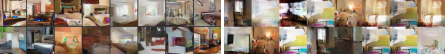
\includegraphics[scale=0.7]{chapter_14/files/wgan_improved.png}
  \caption{Generated images using WGAN (left) vs GAN (right) algorithms, with the same architecture. Note mode collapse for the GAN images. Images from \cite{arjovsky2017wasserstein}}
\end{figure}